\section{How much does $\beta$ affect the performance?}
In order to investigate the performance of \textsf{SGL} as a function of $\beta$, we take grid graph
setting and vary $\beta$ for different regimes of sample size.

Figure~\ref{fig:performance-beta} depicts the performance.

\begin{figure}[!htb]
    \centering
    \begin{subfigure}[b]{0.47\textwidth}
        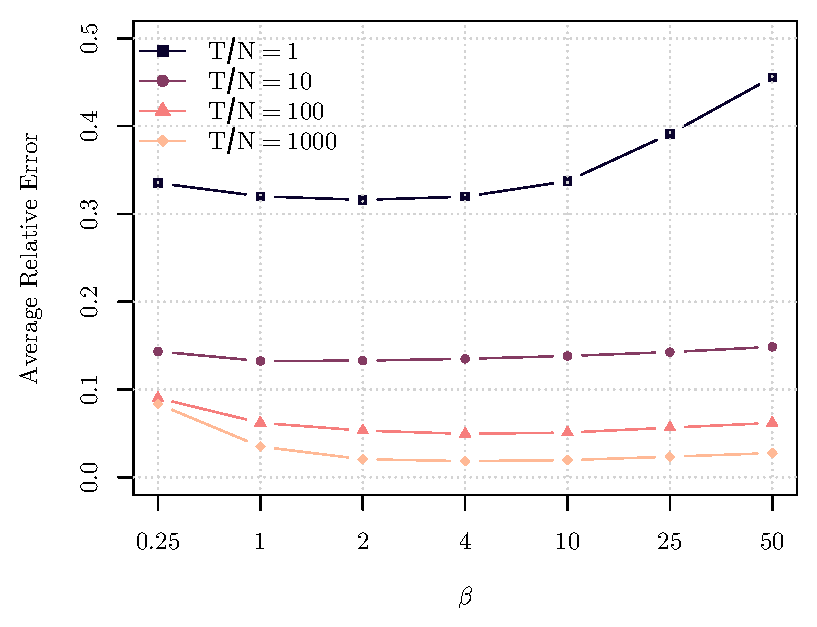
\includegraphics[width=\textwidth]{beta-eval/relative_error_beta.eps}
    \end{subfigure}
    ~ %add desired spacing between images, e. g. ~, \quad, \qquad, \hfill etc.
      %(or a blank line to force the subfigure onto a new line)
    \begin{subfigure}[b]{0.47\textwidth}
        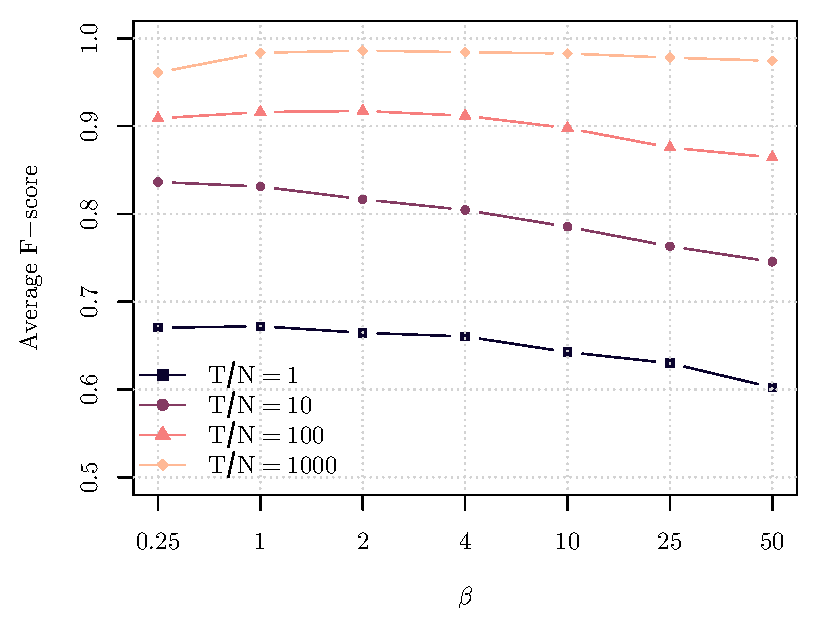
\includegraphics[width=\textwidth]{beta-eval/fscore_beta.eps}
    \end{subfigure}
    \caption{Average performance results for learning Laplacian matrix of a $\mathcal{G}^{(64, 0.1)}_{\mathsf{grid}}$.}
    \label{fig:performance-beta}
\end{figure}

